% =============================================================
%  CAPÍTULO II — MARCO TEÓRICO DEL PROYECTO TECNOLÓGICO
% =============================================================

\section{Marco conceptual}

En el contexto de las evaluaciones por competencia curricular, los métodos de evaluación juegan un papel crucial. Estos métodos son los enfoques y herramientas utilizados para medir el grado en que los estudiantes han adquirido las competencias específicas delineadas en el plan de estudios, pudiendo abarcar desde pruebas tradicionales hasta proyectos prácticos, pasando por evaluaciones basadas en la resolución de problemas o en la presentación oral \cite{black1998inside,voinea2025competency}.

La \textbf{competencia}, en este contexto, se refiere a la capacidad demostrada por un estudiante para aplicar conocimientos, habilidades y actitudes de manera efectiva y apropiada en situaciones específicas. En lugar de simplemente memorizar información, la competencia implica la capacidad de utilizar ese conocimiento de manera significativa y transferible en el mundo real \cite{oecd2019compass}. La literatura actual distingue entre competencias cognitivas, interactivas y afectivas, todas ellas evaluables a través de instrumentos diseñados con criterios auténticos \cite{voinea2025competency}.

El \textbf{aprendizaje individualizado} es un enfoque educativo que reconoce las diferencias entre los estudiantes y adapta el proceso de enseñanza para satisfacer las necesidades únicas de cada uno \cite{sayed2023adaptive}. En plataformas tecnológicas actuales, este principio se operacionaliza mediante motores adaptativos que ajustan la dificultad de los contenidos y la secuencia de tareas en función del desempeño individual, reduciendo la brecha entre la instrucción homogénea y las necesidades reales del aula \cite{evans2020cbe}.

La \textbf{retroalimentación significativa} se refiere a los comentarios proporcionados a los estudiantes después de una evaluación con el propósito de guiar su aprendizaje de manera efectiva. En el contexto de las evaluaciones por competencia curricular, la retroalimentación significativa no solo señala errores, sino que identifica áreas de mejora, ofrece orientación concreta sobre cómo avanzar y fomenta la autorregulación del estudiante \cite{hattie2007feedback}. El meta-análisis seminal de Hattie y Timperley \cite{hattie2007feedback} demostró que la retroalimentación oportuna tiene uno de los mayores efectos sobre el rendimiento académico de entre todas las intervenciones pedagógicas documentadas, con un tamaño del efecto promedio de $d = 0.79$.

La \textbf{accesibilidad cognitiva} constituye otra dimensión esencial en el diseño de herramientas evaluativas para niños. La discapacidad intelectual y otras condiciones que afectan la comprensión, el procesamiento y la retención de información demandan instrumentos que reduzcan la carga cognitiva mediante apoyos visuales y simbólicos \cite{mayer2014multimedia,guillomia2021cognitive}. En este sentido, el uso de pictogramas —especialmente los provenientes de bases validadas clínicamente como ARASAAC— ha demostrado mejorar la comprensión autónoma y reducir la dependencia de la lectoescritura en contextos de evaluación infantil \cite{guillomia2021cognitive}.

El \textbf{currículum}, también conocido como plan de estudios, proporciona el marco sobre el cual se basan las evaluaciones, delineando las competencias que se espera que los estudiantes adquieran y demuestren durante su proceso educativo \cite{mineduc2021curriculo}. En Ecuador, el Currículo Priorizado del MINEDUC estructura el área de Matemáticas en torno a destrezas con criterio de desempeño que requieren evaluaciones auténticas, continuas e integradas, y cuya medición efectiva exige instrumentos especializados que van más allá de las pruebas tradicionales de papel y lápiz \cite{velezvelez2024curriculo,velezvelez2024curriculo}.

\subsection{Evolución de las evaluaciones educativas}

El concepto de evaluación ha ido evolucionando en consonancia con los paradigmas educativos predominantes en cada época histórica. Desde una evaluación centrada en el juicio de valor sobre las cosas, se transitó hacia la asignación de valores métricos a objetos educativos, y de allí hacia enfoques sistémicos orientados a la toma de decisiones \cite{maskos2025fa}.

En la década de 1930, Ralph Tyler inauguró el movimiento de la evaluación en función de objetivos formulados con antelación, produciendo un cambio paradigmático que desplazó el foco desde la inspección del proceso hacia la verificación de resultados de aprendizaje. En los años sesenta, la evaluación se redefinió como una etapa de ``recopilación y uso de información para tomar decisiones sobre un programa educativo'' \cite{black1998inside}, transformando la percepción del examen como instrumento de control hacia la de un mecanismo de retroalimentación continua. A inicios del siglo~XXI, se consolida una concepción ecléctica que define la evaluación como el proceso de delinear, obtener, procesar y proporcionar información válida, confiable y oportuna para juzgar el mérito de programas y orientar decisiones \cite{maskos2025fa}.

En la actualidad, la investigación coincide en que la evaluación debe atender no solo los resultados cognitivos sino también los no cognitivos, incluyendo motivación, autorregulación y actitudes hacia el aprendizaje \cite{maskos2025fa}. La revisión sistemática de Hagenauer et al. \cite{maskos2025fa}, que analizó 45 estudios publicados entre 2015 y 2023, constata que las evaluaciones computacionales en entornos interactivos presentan un potencial particularmente prometedor, especialmente cuando se implementan de forma regular con instrumentos alineados al contenido específico.

\subsection{Evaluación por competencias}

La evaluación por competencias implica la recopilación de evidencias mediante actividades de aprendizaje y la formulación de valoraciones sobre el progreso del estudiante en relación con los resultados de aprendizaje esperados \cite{voinea2025competency,oecd2019compass}. El autor considera que este enfoque representa un cambio estructural profundo: no se trata únicamente de modificar los instrumentos de medición, sino de replantear la función misma de la evaluación dentro del proceso educativo, reconociéndola como un componente integral del aprendizaje y no como un evento terminal.

La evaluación por competencias ofrece nuevas oportunidades a los estudiantes al generar entornos significativos de aprendizaje que acercan sus experiencias académicas al mundo real \cite{evans2020cbe}. Las competencias evaluadas se componen de estructuras de conocimiento, habilidades cognitivas, interactivas y afectivas, actitudes y valores, necesarios para la ejecución eficaz de tareas en contextos auténticos \cite{voinea2025competency}. La revisión sistemática de Evans et al. \cite{evans2020cbe}, que analizó investigaciones sobre educación basada en competencias en K-12 desde el año 2000 hasta 2019, identificó que las prácticas asociadas a mejores resultados incluyen la definición clara de expectativas de desempeño y el uso de múltiples tipos de evaluación para verificar el dominio competencial.

\subsection{Evaluación por competencias en matemáticas}

La competencia matemática es un tema de alta relevancia en los países que han adoptado el enfoque competencial para la enseñanza de esta disciplina \cite{maskos2025fa,oecd2023pisa}. Este enfoque demanda reemplazar un currículo centrado únicamente en la adquisición de contenidos por uno que se centre en la alfabetización matemática, permitiendo a los estudiantes utilizar el conocimiento matemático de manera efectiva en diversas situaciones cotidianas \cite{oecd2023pisa}.

La competencia matemática implica la capacidad de dar un uso funcional al conocimiento matemático desde una comprensión profunda \cite{oecd2019compass}. Los estudiantes, al enfrentarse a problemas en contextos del mundo real, deben activar competencias matemáticas pertinentes: analizar, razonar, comunicar y resolver problemas matemáticos en situaciones que involucran conceptos cuantitativos, espaciales o probabilísticos. El desarrollo de esta competencia no tiene un punto final; es un proceso continuo en el que cada nueva situación amplía el dominio competencial del estudiante \cite{maskos2025fa}.

Los resultados del PISA 2022 \cite{oecd2023pisa} constituyen una advertencia empírica contundente: el rendimiento medio en matemáticas en los países de la OCDE cayó 15 puntos entre 2018 y 2022, la mayor caída registrada históricamente. En América Latina y el Caribe, tres de cada cuatro estudiantes no alcanzan el nivel mínimo de competencia matemática \cite{bid2023pisa,unesco2024lac}, lo que impone una responsabilidad urgente al diseño de instrumentos evaluativos especializados para los primeros ciclos de formación.

\subsection{Tipos de preguntas en evaluaciones por competencias}

En la evaluación por competencias, el diseño de preguntas juega un papel crucial para medir de manera efectiva las habilidades y conocimientos que se buscan evaluar \cite{evans2020cbe}. Estas preguntas trascienden la memorización para evidenciar la aplicación práctica de conocimientos y habilidades en situaciones del mundo real. La literatura especializada identifica las siguientes categorías como las más empleadas en este enfoque:

\begin{itemize}[leftmargin=*]
  \item \textbf{Preguntas de Aplicación:} Desafían a los evaluados a aplicar conocimientos y habilidades en situaciones prácticas, poniendo a prueba la transferencia del conocimiento adquirido.
  \item \textbf{Estudios de Caso:} Presentan un escenario detallado y piden al evaluado que analice, interprete y proponga soluciones fundamentadas en sus conocimientos previos.
  \item \textbf{Problemas de Resolución:} Requieren que el estudiante resuelva situaciones problemáticas utilizando habilidades matemáticas, lógicas o procedimentales.
  \item \textbf{Preguntas Situacionales:} Presentan situaciones hipotéticas o reales y demandan decisiones o soluciones basadas en el conocimiento y la experiencia del evaluado.
\end{itemize}

Estos tipos de preguntas permiten medir habilidades como el pensamiento crítico, la resolución de problemas, la toma de decisiones y la capacidad de operar en situaciones del mundo real \cite{mayer2014multimedia}. El autor señala que, en el contexto de la educación básica elemental, el diseño de preguntas debe incorporar adicionalmente criterios de accesibilidad cognitiva, de modo que la carga lingüística del enunciado no condicione negativamente el desempeño de los estudiantes que aún consolidan sus habilidades lectoras.

\subsection{Integración de diferentes tipos de preguntas}

La integración de diversos tipos de preguntas en una evaluación es fundamental para capturar de manera integral las habilidades y conocimientos de los estudiantes \cite{evans2020cbe,maskos2025fa}. Al combinar preguntas de aplicación, estudios de caso, problemas de resolución y preguntas situacionales, se abarcan diferentes niveles de comprensión taxonómica y se evalúan habilidades específicas, desde la aplicación práctica hasta el pensamiento crítico.

Esta diversidad no solo se adapta a diferentes estilos de aprendizaje, sino que también proporciona a los educadores una perspectiva más completa del rendimiento estudiantil, habilitando decisiones pedagógicas más informadas \cite{maskos2025fa}. La integración de distintos tipos de preguntas impulsa a los estudiantes a aplicar, analizar y tomar decisiones, promoviendo un aprendizaje significativo orientado al desarrollo de competencias genuinas y no solo a la reproducción de contenidos memorizados \cite{hattie2007feedback}.

\subsection{Uso de elementos multimedia en preguntas educativas}

La inclusión de elementos multimedia en las evaluaciones dirigidas a niños desempeña un papel crucial en la construcción de un ambiente de aprendizaje estimulante y accesible \cite{mayer2014multimedia}. La Teoría Cognitiva del Aprendizaje Multimedia, propuesta por Mayer \cite{mayer2014multimedia}, establece que los seres humanos aprenden más profundamente a partir de imágenes y palabras combinadas que a partir de palabras solas, dado que el procesamiento visual y verbal operan en canales cognitivos distintos que, utilizados conjuntamente, potencian la comprensión y la retención.

La incorporación de imágenes, pictogramas e íconos adaptados a la edad no solo captura la atención de los niños, sino que reduce la carga cognitiva extrínseca y facilita la comprensión de conceptos abstractos, promoviendo una experiencia de evaluación más equitativa para estudiantes con diferentes niveles de lectoescritura \cite{mayer2014multimedia,guillomia2021cognitive}. Investigaciones recientes sobre comunicación aumentativa y alternativa (CAA) confirman que los pictogramas provenientes de repositorios validados como ARASAAC presentan una cobertura semántica superior al 95\,\% en cinco idiomas, con calificaciones de adecuación visual reportadas como correctas o aceptables por evaluadores clínicos expertos \cite{guillomia2021cognitive}.

\subsection{La tecnología educativa}

La tecnología educativa se ocupa del análisis de los medios, materiales, plataformas y entornos digitales utilizados en los procesos de aprendizaje \cite{sayed2023adaptive}. Lejos de ser un fenómeno nuevo, la vinculación entre educación y tecnología es una constante histórica que ha adoptado formas diversas en cada época. Lo que distingue el momento actual es la aceleración del cambio tecnológico y la disponibilidad de herramientas que permiten experiencias de aprendizaje personalizadas, adaptativas y con retroalimentación inmediata a escala masiva \cite{topali2025aied}.

La evidencia empírica respalda de forma consistente que la tecnología, cuando se integra de manera pedagógicamente fundamentada, produce mejoras significativas en el desempeño académico y en la motivación de los estudiantes \cite{debrenti2024gbl,maskos2025fa}. Una revisión sistemática reciente sobre sistemas tutoriales inteligentes (STI) en educación K-12 \cite{mousavinasab2018its}, que analizó 28 estudios con un total de 4.597 estudiantes, encontró que el efecto general de los STI sobre el aprendizaje es positivo, aunque se ve moderado cuando se compara con sistemas tutoriales no inteligentes, lo que subraya la importancia del diseño pedagógico por encima de la sofisticación tecnológica.

\subsection{Aplicaciones educativas}

Las aplicaciones educativas representan herramientas diseñadas para consolidar los conocimientos de los estudiantes en diversas áreas de aprendizaje \cite{sayed2023adaptive,debrenti2024gbl}. Enriquecidas con imágenes, sonidos, animaciones y retroalimentación interactiva adaptadas a las distintas edades y disciplinas, estas aplicaciones constituyen un recurso de creciente centralidad en los sistemas educativos contemporáneos. La investigación comparativa sobre aplicaciones matemáticas para educación primaria \cite{outhwaite2022apps} ha evidenciado que las apps que abarcan un currículo matemático más amplio reportan mayores resultados de aprendizaje que las enfocadas en habilidades aisladas, incluyendo beneficios en atención y generalización a medidas secundarias.

El autor destaca que la efectividad de las aplicaciones educativas no es inherente a su existencia, sino que depende de su alineación curricular, su diseño de interfaz, la calidad de la retroalimentación que proveen y su capacidad de adaptarse a los ritmos individuales de aprendizaje \cite{sayed2023adaptive,vlachogianni2022sus}. La revisión sistemática de Vlachogianni y Tselios \cite{vlachogianni2022sus}, publicada en el \textit{Journal of Research on Technology in Education}, constató que las evaluaciones de usabilidad percibida mediante SUS en tecnología educativa muestran puntuaciones promedio consistentemente superiores al umbral de 68 puntos cuando el diseño de la interfaz respeta los principios de usabilidad pediátrica y de accesibilidad cognitiva.

\subsection{Desarrollo de aplicaciones para evaluación educativa}

La importancia de las aplicaciones educativas orientadas a la evaluación radica en su capacidad para proporcionar experiencias interactivas y personalizadas que van más allá de la medición puntual \cite{gonzalez2021ai,maksimchuk2025genai}. Al incorporar elementos visuales, auditivos y táctiles, estas aplicaciones estimulan la participación activa, fomentan un ambiente más dinámico y ofrecen la flexibilidad necesaria para adaptarse a diversos estilos de aprendizaje \cite{sayed2023adaptive}.

La selección adecuada de tecnologías de desarrollo es determinante para garantizar la eficacia, la seguridad y la escalabilidad del sistema resultante \cite{dyba2008agile}. Para el desarrollo de Kiddy Quiz, se seleccionaron tecnologías ampliamente validadas en la industria: Angular, reconocido por su robustez en la creación de interfaces de usuario interactivas y su capacidad para desarrollar aplicaciones web progresivas de alto rendimiento; NestJS, que centraliza la lógica del \textit{backend} bajo una arquitectura modular inspirada en los principios de diseño orientado a objetos; y PostgreSQL como motor de base de datos relacional, que garantiza un almacenamiento estructurado, eficiente y escalable con integridad referencial. Esta arquitectura se complementa con la API generativa Gemini~2.5 Flash para la retroalimentación inteligente y Cloudinary para la gestión optimizada de recursos multimedia, conformando una solución tecnológica cohesiva y de nivel productivo.

\subsection{Programación Extrema (XP)}

La Programación Extrema (XP) es una metodología ágil de desarrollo de software que se enfoca en la entrega rápida de valor al cliente mediante iteraciones cortas y prácticas técnicas rigurosas \cite{beck2004xp}. XP es independiente de herramientas o lenguajes particulares, brindando a los equipos la flexibilidad para construir software de alta calidad en entornos de alta incertidumbre y con requisitos cambiantes, condición inherente a los proyectos de software educativo \cite{dyba2008agile}.

Las prácticas de XP se fundamentan en valores como la comunicación constante, la simplicidad del diseño y el coraje para refactorizar continuamente el sistema \cite{beck2004xp}. La revisión sistemática de Dybå y Dingsøyr \cite{dyba2008agile}, publicada en \textit{Information and Software Technology} (Q1, JCR), confirma que los métodos ágiles —y XP en particular— producen mejoras consistentes en la calidad del código, la satisfacción del cliente y la capacidad de respuesta ante cambios de requisitos, en comparación con metodologías en cascada. De manera complementaria, Shrivastava et al. \cite{shrivastava2021xpreview} concluyen en su revisión sistemática que XP es especialmente adecuada para equipos pequeños o individuales que trabajan en proyectos con alta interacción con el usuario final, contexto que describe con precisión el desarrollo de Kiddy Quiz.

A continuación, se describen las cuatro fases principales del ciclo de desarrollo XP propuesto por Pressman \cite{beck2004xp}:

\begin{itemize}[leftmargin=*]
  \item \textbf{Fase de Planeación:} Mediante el Juego de Planificación, el cliente presenta necesidades en forma de Historias de Usuario, las cuales son estimadas y priorizadas por el equipo de desarrollo. La presencia activa del cliente en el sitio es fundamental para resolver dudas y validar decisiones de manera ágil.
  \item \textbf{Fase de Diseño:} La prioridad es mantener el Diseño Simple, buscando siempre la solución más sencilla que cumpla con los requisitos actuales, evitando la complejidad innecesaria y la anticipación de funcionalidades futuras que podrían no materializarse.
  \item \textbf{Fase de Codificación:} El Desarrollo Dirigido por Pruebas (TDD) guía la implementación: se escriben pruebas automatizadas antes del código funcional. La Refactorización continua mejora la estructura interna del código sin alterar su comportamiento externo, manteniendo el sistema limpio y mantenible.
  \item \textbf{Fase de Prueba y Entrega:} Los Lanzamientos Pequeños proveen versiones funcionales al cliente con alta frecuencia, habilitando retroalimentación temprana y alimentando las siguientes iteraciones de desarrollo con evidencia real de uso.
\end{itemize}

% =============================================================
\subsection{Accesibilidad e inclusión en el software educativo}

En el ámbito de la ingeniería de software educativo, la inclusión
trasciende la mera disponibilidad técnica; implica la creación de
entornos que eliminen las barreras de aprendizaje y participación.
Para que una aplicación sea considerada verdaderamente inclusiva, debe
ser diseñada bajo principios que reconozcan la diversidad de
capacidades cognitivas y sensoriales de los usuarios
\cite{unesco2017inclusion}. En el caso de Kiddy Quiz, esta visión
se operacionaliza a través de dos pilares fundamentales: el marco
pedagógico del Diseño Universal para el Aprendizaje (DUA) y los
estándares técnicos de las Pautas de Accesibilidad para el Contenido
Web (WCAG).

\subsubsection{Diseño Universal para el Aprendizaje (DUA)}

El Diseño Universal para el Aprendizaje (DUA) se define como un marco
que busca minimizar las barreras y maximizar el aprendizaje para todo
el alumnado \cite{rose2002udl}. El Ministerio de Educación del Ecuador
impulsa igualmente este enfoque como eje transversal del sistema
educativo nacional \cite{mineduc2023dua}. Su aplicación en esta
plataforma permite que la evaluación de competencias matemáticas sea un
proceso flexible y no rígido, alineado con sus tres principios
fundamentales:

\begin{enumerate}[leftmargin=*]
  \item \textbf{Múltiples medios de representación:} Al integrar texto,
  pictogramas y síntesis de voz, se ofrece la información a través de
  diferentes canales sensoriales. Esto garantiza que el contenido sea
  accesible tanto para estudiantes con lectura fluida como para quienes
  dependen de apoyos visuales o auditivos.

  \item \textbf{Múltiples medios de acción y expresión:} La interfaz
  permite al estudiante interactuar con las evaluaciones de forma
  intuitiva, de modo que pueda demostrar sus conocimientos matemáticos
  sin que la complejidad de la navegación digital constituya un
  obstáculo.

  \item \textbf{Múltiples medios de compromiso:} La retroalimentación
  inmediata generada por IA y el refuerzo auditivo incrementan la
  motivación y la autonomía, factores determinantes para mantener la
  atención en estudiantes con perfiles de aprendizaje diversos.
\end{enumerate}

\subsubsection{Criterios de accesibilidad web (WCAG)}

Para garantizar la viabilidad técnica de la inclusión, el desarrollo
de la aplicación se fundamenta en las Pautas de Accesibilidad para el
Contenido Web (WCAG 2.1). Estas directrices internacionales aseguran
que el contenido sea perceptible, operable, comprensible y robusto
\cite{w3c2018wcag}.

En concreto, se priorizaron criterios como el contraste visual adecuado
entre texto y fondo para facilitar la lectura, la legibilidad mediante
tipografías claras y espaciado óptimo, y la provisión de alternativas
de audio y texto para todos los elementos no textuales (como los botones
de acción). Estas implementaciones aseguran que la plataforma sea
funcional para la mayor variedad posible de usuarios, incluyendo
aquellos con discapacidades visuales leves o dificultades de
procesamiento perceptivo.

\subsubsection{Fundamentación de los pictogramas y neurodiversidad}

El uso de pictogramas en la plataforma no es una elección meramente
estética, sino una herramienta validada de Comunicación Aumentativa y
Alternativa (CAA). Teóricamente, el apoyo visual reduce la carga
cognitiva y facilita la construcción de modelos mentales más claros,
lo cual resulta determinante en las etapas iniciales de la
lectoescritura \cite{mayer2014multimedia,guillomia2021cognitive}.

Más allá de la etapa de alfabetización, el uso sistemático de apoyos
visuales constituye una estrategia de inclusión eficaz para estudiantes
con neurodivergencias, tales como el Trastorno por Déficit de Atención
con Hiperactividad (TDAH), dislexia o Trastorno del Espectro Autista
(TEA). Para estos estudiantes, los pictogramas proporcionan una
estructura predecible y una comprensión inmediata del concepto
matemático, permitiendo que la evaluación mida realmente su competencia
en la asignatura y no su capacidad de descodificación de textos extensos
\cite{zurita2026arasaac,guillomia2021cognitive}. Es precisamente esta
capacidad de adaptación a la diversidad cognitiva la que justifica y
fundamenta la categorización de Kiddy Quiz como
\textit{``Aplicación Web Inclusiva''}.

% =============================================================
\section{Marco referencial}
% =============================================================
\label{sec:marco-referencial}

El marco referencial complementa el sustento teórico del proyecto mediante el análisis crítico de iniciativas previas que han abordado, total o parcialmente, la problemática de la evaluación formativa por competencias mediada por tecnología en educación básica. A diferencia del marco conceptual ---orientado a precisar las nociones que estructuran el estudio---, el presente apartado examina la evidencia empírica acumulada sobre herramientas, plataformas y arquitecturas tecnológicas efectivamente desplegadas en contextos educativos reales. Este ejercicio responde a un principio metodológico esencial en investigación tecnológica aplicada: ningún desarrollo de software educativo debería concebirse al margen del estado del arte, pues solo a partir de la identificación de logros consolidados, brechas persistentes y oportunidades aún no atendidas resulta posible justificar de manera rigurosa la pertinencia y la novedad de una nueva propuesta. En consecuencia, el análisis que se presenta a continuación cumple una doble función: por un lado, sitúa a Kiddy Quiz dentro de la trayectoria internacional de soluciones tecnológicas para la evaluación educativa; por otro, evidencia los vacíos específicos que el proyecto busca atender, particularmente en lo concerniente a la educación básica elemental, dimensión sistemáticamente subrepresentada en la literatura de referencia.

\subsection{Análisis del estado del arte sobre herramientas tecnológicas de evaluación en educación primaria}
\label{subsec:estado-arte}

La evaluación formativa mediada por tecnología en educación básica ha generado, en años recientes, un cuerpo creciente de investigación que documenta tanto avances metodológicos como brechas instrumentales persistentes. Con el propósito de fundamentar empíricamente la propuesta del presente proyecto, se realizó una revisión exploratoria del estado del arte sobre plataformas y herramientas tecnológicas para la evaluación educativa, priorizando publicaciones académicas indexadas en \textit{Web of Science Core Collection} dentro del período 2017--2026.

\subsubsection{Protocolo de búsqueda}

La búsqueda se ejecutó mediante consultas estructuradas con el operador \textit{TS} (\textit{Topic}: title, abstract, author keywords y \textit{KeyWords Plus}), aplicando expansión por sinónimos y truncamiento (\texttt{*}) para maximizar la cobertura terminológica. Las siete cadenas ejecutadas fueron las siguientes:

\begin{enumerate}
\item Búsqueda general por evaluación basada en competencias en educación primaria:
\begin{Verbatim}[fontsize=\footnotesize, xleftmargin=1.5em]
TS=(competency-based assessment) AND TS=(elementary education)
\end{Verbatim}

\item Evaluación formativa digital aplicada a matemáticas de primaria:
\begin{Verbatim}[fontsize=\footnotesize, xleftmargin=1.5em]
TS=("digital formative assessment") AND TS=(primary school mathematics)
\end{Verbatim}

\item Analítica del aprendizaje en educación primaria:
\begin{Verbatim}[fontsize=\footnotesize, xleftmargin=1.5em]
TS=("learning analytics") AND TS=("primary education")
\end{Verbatim}

\item Software educativo, usabilidad infantil y matemáticas:
\begin{Verbatim}[fontsize=\footnotesize, xleftmargin=1.5em]
TS=("educational software") AND TS=(usability children mathematics)
\end{Verbatim}

\item Pictogramas y símbolos visuales en evaluación educativa infantil:
\begin{Verbatim}[fontsize=\footnotesize, xleftmargin=1.5em]
TS=(pictograms OR "visual symbols" OR "graphic symbols")
   AND TS=("educational assessment" OR "formative assessment"
           OR evaluation)
   AND TS=(children OR "primary school" OR "elementary education")
\end{Verbatim}

\item Inteligencia artificial generativa y retroalimentación formativa en K--12:
\begin{Verbatim}[fontsize=\footnotesize, xleftmargin=1.5em]
TS=("generative AI" OR "generative artificial intelligence"
    OR "GenAI" OR ChatGPT OR LLM OR "large language model")
   AND TS=(feedback OR retroalimentaci*)
   AND TS=("formative assessment" OR "formative evaluation")
   AND TS=("K-12" OR "primary school" OR "secondary school"
           OR "elementary education" OR "school education")
\end{Verbatim}

\item Herramientas y plataformas web de evaluación por competencias:
\begin{Verbatim}[fontsize=\footnotesize, xleftmargin=1.5em]
TS=("competency assessment tool" OR "competency assessment platform"
    OR "competence assessment tool" OR "competency-based assessment")
   AND TS=("web platform" OR "web application"
           OR "web-based" OR "online platform")
   AND TS=(evaluation OR validation OR usability)
\end{Verbatim}
\end{enumerate}

El proceso de selección de los estudios incluidos en la síntesis siguió un flujo adaptado del protocolo PRISMA \cite{page2021prisma}, garantizando trazabilidad y reproducibilidad de la revisión. La Figura~\ref{fig:prisma} sintetiza el flujo completo: las siete cadenas arrojaron noventa registros iniciales en \textit{Web of Science Core Collection}; tras la eliminación de duplicados y el cribado por título y resumen, sesenta registros pasaron a la fase de evaluación de elegibilidad mediante lectura completa; trece estudios fueron descartados por contexto no aplicable a primaria o por insuficiente rigor metodológico, conformándose finalmente un corpus de \textbf{veintidós trabajos} que constituye la base empírica del análisis presentado en las siguientes subsecciones.

\begin{figure}[H]
\centering
\footnotesize
\begin{tikzpicture}[
  node distance=0.5cm and 0.4cm,
  base/.style={draw, rectangle, rounded corners=2pt, align=center,
               minimum height=1.1cm, text width=6.2cm, font=\footnotesize, inner sep=4pt},
  fase/.style={draw, rectangle, fill=gray!15, rounded corners=2pt,
               align=center, minimum height=1.1cm, text width=2.0cm,
               font=\footnotesize\bfseries, inner sep=4pt},
  excl/.style={draw, rectangle, dashed, align=center, minimum height=1.1cm,
               text width=4.8cm, font=\footnotesize, fill=gray!5, inner sep=4pt},
  arr/.style={-{Stealth[length=2mm]}, thick}
]

\node[fase] (f1) {IDENTIFI-\\CACI\'ON};
\node[fase, below=2.0cm of f1] (f2) {CRIBADO};
\node[fase, below=2.0cm of f2] (f3) {ELEGIBI-\\LIDAD};
\node[fase, below=1.5cm of f3] (f4) {INCLUSI\'ON};

\node[base, right=of f1] (n1) {Registros identificados en \textit{Web of Science} mediante 7 cadenas de búsqueda\\ \textbf{(n = 90)}};
\node[base, right=of f2] (n2) {Registros tras eliminación de duplicados y cribado por título y resumen\\ \textbf{(n = 60)}};
\node[base, right=of f3] (n3) {Estudios evaluados para elegibilidad por lectura completa\\ \textbf{(n = 35)}};
\node[base, right=of f4] (n4) {Estudios incluidos en la síntesis cualitativa\\ \textbf{(n = 22)}};

\node[excl, right=of n1] (e1) {Duplicados eliminados\\ \textbf{(n = 30)}};
\node[excl, right=of n2] (e2) {Excluidos por irrelevancia temática: medicina, salud, educ.\ superior, política\\ \textbf{(n = 25)}};
\node[excl, right=of n3] (e3) {Excluidos por contexto no aplicable a primaria o por insuficiente rigor metodológico\\ \textbf{(n = 13)}};

\draw[arr] (n1) -- (n2);
\draw[arr] (n2) -- (n3);
\draw[arr] (n3) -- (n4);
\draw[arr] (n1) -- (e1);
\draw[arr] (n2) -- (e2);
\draw[arr] (n3) -- (e3);
\end{tikzpicture}
\caption{Diagrama de flujo del proceso de selección de estudios siguiendo el protocolo PRISMA adaptado.}
\label{fig:prisma}
\end{figure}
\elaboracion

\noindent El corpus resultante se organizó analíticamente en cinco ejes temáticos derivados inductivamente del propio contenido de los trabajos: (i) evaluación formativa digital y \textit{learning analytics} en primaria; (ii) sistemas de evaluación adaptativa; (iii) inteligencia artificial generativa para retroalimentación formativa; (iv) gamificación y motivación; y (v) accesibilidad cognitiva mediante pictogramas. Esta organización temática permite, en las siguientes subsecciones, sintetizar los principales aportes de cada eje y, simultáneamente, identificar las limitaciones que la propuesta Kiddy Quiz busca superar.

\subsubsection{Evaluación formativa digital y \textit{learning analytics} en educación primaria}

Este eje concentra la evidencia más sólida y de mayor impacto bibliométrico relativa al objeto de estudio. La plataforma \textit{Snappet}, desplegada en escuelas primarias de los Países Bajos, ha sido objeto de dos estudios complementarios que, en conjunto, constituyen la evidencia experimental más robusta sobre evaluación formativa digital en este nivel educativo. Por una parte, Faber, Luyten y Visscher \cite{faber2017dfa}, en \textit{Computers \& Education}, demostraron mediante un experimento aleatorizado con 79 escuelas y 1\,808 estudiantes de tercer grado que la integración en una herramienta digital de retroalimentación al estudiante, retroalimentación al docente y asignaciones adaptativas produce efectos positivos significativos sobre el rendimiento matemático y la motivación, especialmente intensos entre estudiantes de alto desempeño previo.

Complementariamente, Molenaar y Knoop-van Campen \cite{molenaar2016snappet} ---en estudio cuasi-ex\-pe\-ri\-men\-tal publicado en las actas de la conferencia LAK--- caracterizaron a Snappet como tecnología que combina \textit{learning analytics} extraída ---panel de control en tiempo real para el docente--- con \textit{learning analytics} embebida ---ajuste automático de la dificultad de los ejercicios---, mostrando progresos significativamente superiores en habilidades aritméticas para estudiantes de cuarto grado, con beneficios marginales mayores entre los de alto rendimiento.

\textbf{Limitaciones frente a la propuesta:} Snappet se concentra en bancos cerrados de ejercicios estandarizados ---fundamentalmente aritméticos y ortográficos--- provistos por la plataforma; no contempla la creación de instrumentos por parte del docente regular, ni apoyos pictográficos para accesibilidad cognitiva, ni retroalimentación generativa. Kiddy Quiz amplía el alcance hacia la evaluación curricular alineada con el currículo ecuatoriano y combina las ventajas analíticas de Snappet con un editor docente para creación heterogénea de ítems y con generación automática de retroalimentación motivacional.

Los estudios del grupo de Tirado-Olivares y colaboradores en la Universidad de Castilla-La Mancha conforman una de las líneas de investigación más productivas a nivel internacional sobre \textit{learning analytics} aplicada a evaluación formativa en primaria. Tirado-Olivares, López-Fernández, González-Calero y Cózar-Gutiérrez \cite{tirado2024analytics} documentaron, con 76 estudiantes de 10--12 años, que la integración de \textit{learning analytics} en la enseñanza del pensamiento histórico mejora especialmente el rendimiento académico de estudiantes con bajo conocimiento histórico previo, y revelan disparidades entre el conocimiento real, la autoeficacia percibida y el desempeño en exámenes ---hallazgo que justifica la inclusión de actividades formativas previas a la evaluación sumativa---. En un estudio paralelo, Tirado-Olivares et al.\ \cite{tirado2024lms} evaluaron en \textit{Sustainability} el impacto de sistemas de gestión del aprendizaje en educación geográfica primaria, evidenciando que la retroalimentación basada en \textit{learning analytics} es un factor explicativo central de las ganancias observadas. Más recientemente, Tirado-Olivares, Mínguez-Pardo y del Olmo-Muñoz \cite{tirado2025bridge} confirmaron, con 235 estudiantes de quinto y sexto grado y mediante diseño con tres condiciones experimentales (ejemplos correctos, ejemplos erróneos, sin tareas), que las tareas basadas en ejemplos correctos integradas con \textit{learning analytics} mejoran significativamente el aprendizaje de números decimales, particularmente entre estudiantes con menor conocimiento previo. Complementariamente, Rodríguez-Martínez et al.\ \cite{rodriguez2023personalised}, en \textit{British Journal of Educational Technology}, demostraron con 127 estudiantes españoles de quinto grado que la construcción de tareas personalizadas a partir de evaluaciones formativas basadas en \textit{learning analytics} mejora la comprensión de fracciones de manera significativa frente a tareas genéricas idénticas para todos los estudiantes. \textbf{Limitaciones frente a la propuesta:} los cuatro estudios operan sobre la plataforma Moodle u otros entornos investigativos y dependen de bancos de tareas curados externamente por el equipo investigador; ninguno reporta funcionalidad para que el docente regular cree instrumentos de manera autónoma. Kiddy Quiz internaliza la creación de evaluaciones en una interfaz docente diseñada para uso autónomo del profesorado.

Mohseni y Masiello \cite{mohseni2025mlad}, de la Universidad de Linnaeus (Suecia), presentan en \textit{Educational Technology Research and Development} los Múltiples Paneles de Analítica del Aprendizaje (MLAD, por sus siglas en inglés \textit{Multiple Learning Analytics Dashboards}) desarrollados mediante metodología de investigación basada en diseño con docentes de tres municipios suecos seleccionados por sus diferencias en infraestructura digital, plataformas de gestión del aprendizaje y demografía estudiantil. La contribución central es metodológica: identificar requisitos mediante entrevistas con \textit{stakeholders}, generar ideas mediante \textit{brainstorming} y prototipado, codiseñar y validar la usabilidad con docentes, y finalmente implementar los paneles en entornos reales. \textbf{Limitaciones frente a la propuesta:} MLAD es exclusivamente un sistema de visualización analítica; no incluye módulos de creación o aplicación de evaluaciones, ni retroalimentación al estudiante. Kiddy Quiz integra la dimensión analítica de MLAD dentro de una arquitectura más amplia que cubre el ciclo completo de evaluación formativa: creación, aplicación, retroalimentación y analítica.

Bin Qushem, Christopoulos y Laakso \cite{binqushem2022lmsanalytics} analizaron, en \textit{Multimodal Technologies and Interaction}, datos de un sistema de gestión del aprendizaje en una intervención de fluidez aritmética en educación K--6, mostrando que la combinación de analítica conductual y de desempeño permite identificar patrones individuales de progreso. Por su parte, Moltudal, Krumsvik y Høydal \cite{moltudal2022adaptive} en \textit{Frontiers in Education} alertaron, mediante estudio mixto con docentes de primaria superior, que la introducción de tecnología de aprendizaje adaptativo y \textit{learning analytics} en aulas reales genera retos que ``exceden la competencia digital de los docentes'', con efectos sobre la gestión del aula y la profesionalidad docente. Este hallazgo es crítico para el diseño de la interfaz de Kiddy Quiz, cuya prioridad de usabilidad responde explícitamente al perfil de docentes con competencia digital media. Ebner y Schön \cite{ebner2013whymatters}, finalmente, desarrollaron en la Universidad Tecnológica de Graz dos aplicaciones para entrenamiento de competencias en multiplicación que estiman el nivel de competencia del usuario y se adaptan a su desarrollo, argumentando ---con base en datos longitudinales--- la pertinencia de la \textit{learning analytics} en educación primaria, llamado que ha sido respondido empíricamente por los trabajos posteriores aquí reseñados.

\subsubsection{Sistemas de evaluación adaptativa}

Yuhana, Yuniarno, Rahayu y Pardede \cite{yuhana2024adaptive}, en \textit{Education and Information Technologies}, propusieron un modelo de selección contextual de preguntas que extiende el paradigma clásico del \textit{Computerized Adaptive Testing} (CAT) incorporando múltiples aspectos del contexto del usuario. El modelo combina cuatro métodos psicométricos ---\textit{Classical Test Theory}, modelo de Rasch, modelos lineal y cuadrático--- con técnicas de ramificación e ítems adaptativos para seleccionar preguntas de dificultad apropiada para cada estudiante. Su validación con 689 estudiantes de primaria en Indonesia, en el contexto del currículo nacional por competencias, demostró efectividad en la predicción de la apropiación de las preguntas respecto a la habilidad real del estudiante. \textbf{Limitaciones frente a la propuesta:} el modelo opera exclusivamente sobre bancos de preguntas preexistentes y no contempla la generación automática de retroalimentación motivacional; tampoco incluye accesibilidad pictográfica. Kiddy Quiz incorpora elementos de adaptatividad por nivel de dificultad y los complementa con retroalimentación generada por IA y apoyos visuales pictográficos.

Tian, Ding, Tian, Chen y Wang \cite{tian2025intelligent}, en \textit{Assessment in Education: Principles, Policy \& Practice}, desarrollaron un sistema de evaluación inteligente de la habilidad de argumentación científica en estudiantes de sexto grado en China. Comparando cuatro algoritmos de aprendizaje superficial (Naive Bayes Polinomial, k-NN, \textit{Random Forest}, Regresión Logística) y dos modelos de aprendizaje profundo (TextCNN, Bi-LSTM con atención), reportaron que el modelo Bi-LSTM con atención alcanza el 85,87\,\% de precisión y una fuerte consistencia humano-máquina, demostrando aplicabilidad práctica para reducir la carga evaluativa docente. \textbf{Limitaciones frente a la propuesta:} el sistema se especializa en evaluación de argumentación textual mediante procesamiento de lenguaje natural y no aborda la creación flexible de instrumentos por el docente ni la retroalimentación motivacional al estudiante. Kiddy Quiz se sitúa en un enfoque complementario: en lugar de automatizar la evaluación de respuestas abiertas, prioriza la diversidad de tipos de pregunta cerrada con corrección determinista y delega a la IA generativa la dimensión motivacional de la retroalimentación.

Hubálovský, Hubálovská y Musílek \cite{hubalovsky2019adaptive}, en \textit{Computers in Human Behavior}, evaluaron el impacto del aprendizaje electrónico adaptativo en los resultados educativos, evidenciando ganancias de rendimiento cuando los contenidos se ajustan dinámicamente al nivel del estudiante. Cheruiyot y Molnár \cite{cheruiyot2026collaborative}, en \textit{Education and Information Technologies}, ampliaron este paradigma a la evaluación de competencias de resolución colaborativa de problemas científicos mediante adaptación basada en computador. Estos antecedentes consolidan la pertinencia de la adaptatividad como estrategia transversal en evaluación formativa, dimensión incorporada por Kiddy Quiz a nivel de banco de preguntas categorizado por dificultad.

\subsubsection{Inteligencia artificial generativa para retroalimentación formativa}

Este eje constituye la frontera más reciente y dinámica de la investigación en evaluación educativa. Zheng y Tse \cite{zheng2023genai} reportaron, en el congreso IEEE TALE, un estudio de caso con 21 estudiantes de cuarto grado y dos docentes de una escuela primaria china sobre \textit{Class Optimization Master}, un \textit{software} de retroalimentación formativa basada en IA generativa. El análisis temático organizado en torno a las tres dimensiones de la \textit{Mathematical Motivation Scale} ---creencias, compromiso y actitud--- evidenció que la retroalimentación generada por IA mejoró la motivación matemática infantil mediante tres mecanismos: el incremento de la confianza y la promoción de la interacción socioemocional, el refuerzo de la preferencia por las matemáticas, y la estimulación del interés y del esfuerzo mental y físico. Este antecedente es directamente relevante para Kiddy Quiz: valida empíricamente la viabilidad pedagógica de integrar modelos generativos en la evaluación formativa de niños de primaria. \textbf{Limitaciones frente a la propuesta:} el estudio se restringe a un único caso, emplea metodología exclusivamente cualitativa y se centra en la motivación matemática, sin articulación con un marco curricular formal ni evaluación de aceptación tecnológica mediante modelos estandarizados. Kiddy Quiz integra retroalimentación de Gemini~2.5~Flash explícitamente alineada con el Currículo Priorizado con Énfasis en Competencias del Ministerio de Educación del Ecuador, y se valida con SUS y TAM en muestras independientes de docentes y estudiantes.

Fokides y Peristeraki \cite{fokides2025chatgpt}, en \textit{Education and Information Technologies}, compararon la corrección y retroalimentación de ChatGPT con la de educadores humanos sobre redacciones cortas de estudiantes de primaria en inglés y griego. Los autores reportaron que ChatGPT alcanza niveles aceptables de exactitud técnica en la detección de errores pero produce comentarios cualitativamente más genéricos que los del docente experimentado. \textbf{Implicación de diseño para la propuesta:} este hallazgo refuerza la decisión arquitectónica de Kiddy Quiz de \textit{no} sustituir la corrección docente con IA, sino emplear el modelo generativo exclusivamente en la generación de mensajes motivacionales contextualizados a la respuesta del estudiante, dejando la corrección a reglas deterministas verificadas.

Shin, Hwang, Yoo, Bae y Kim \cite{shin2025aigenerated}, en LAK 2025, contrastaron las preferencias estudiantiles entre retroalimentación generada por IA y retroalimentación entre pares en evaluación formativa entre pares, mostrando que la retroalimentación de la IA es valorada por su disponibilidad inmediata, mientras que la de pares aporta dimensiones afectivas que la IA aún no replica plenamente. Banihashem, Bond, Bergdahl, Khosravi y Noroozi \cite{banihashem2025aimapping} ofrecen una revisión sistemática de mapeo en \textit{International Journal of Educational Technology in Higher Education} que identificó 84 estudios sobre IA y aprendizaje autorregulado, concluyendo que la integración de IA en procesos formativos con anclaje pedagógico riguroso es aún una frontera abierta. Bagdonaitė y Dagienė \cite{bagdonaite2025ai}, en \textit{Informatics in Education}, sintetizan en una revisión PRISMA de 94 estudios (2020--2025) que la IA aporta valor máximo en educación primaria cuando \textit{(a)} personaliza retroalimentación y práctica, \textit{(b)} estructura la indagación y el pensamiento computacional y \textit{(c)} potencia la toma de decisiones docente mediante \textit{learning analytics} ---tres dimensiones que Kiddy Quiz integra de forma articulada---. Topali et al.\ \cite{topali2025aied} subrayan, en una revisión sistemática de 28 estudios sobre AIEd en entornos K--12 auténticos, que la mayoría de la investigación se concentra en China y Estados Unidos y se realiza fundamentalmente sobre robots sociales, realidad aumentada y sistemas inteligentes, lo que refuerza la pertinencia de una propuesta validada en Ecuador para diversificar la evidencia empírica del Sur Global.

\subsubsection{Gamificación, motivación y diseño centrado en el estudiante}

Vázquez-Cano, Quicios-García, Fombona y Rodríguez-Arce \cite{vazquezcano2023gamified}, en \textit{Education and Information Technologies}, analizaron mediante modelos de ecuaciones estructurales con 212 docentes españoles los factores latentes de la efectividad educativa de \textit{apps} gamificadas en primaria. Los autores identificaron seis precursores de la efectividad: \textit{(i)} conexión curricular, \textit{(ii)} retroalimentación y experiencia operativa, \textit{(iii)} evaluación e \textit{learning analytics}, \textit{(iv)} sostenibilidad y protección de datos, \textit{(v)} acceso equitativo, y \textit{(vi)} fluidez (\textit{flow}). \textbf{Implicación de diseño para la propuesta:} estos seis precursores fueron utilizados como criterios de diseño explícitos en la arquitectura de Kiddy Quiz, particularmente en la conexión curricular ecuatoriana, la integración de \textit{learning analytics} consultable por el docente, y la implementación de mecánicas de \textit{flow} mediante niveles de dificultad progresiva.

Castro, Sevillano y Cadavieco \cite{castro2024seriousgames,castro2023seriousgames} ampliaron esta línea investigando el impacto de \textit{serious games} sobre la competencia lingüística en educación primaria, confirmando los hallazgos de Vázquez-Cano respecto al rol de la gamificación como mediador motivacional. Amran, Ahmad y Nayan \cite{amran2021design}, en \textit{International Journal of Technology Enhanced Learning}, demostraron mediante diseño participativo con once estudiantes de 8 a 12 años que la inclusión de niños como socios de diseño produce \textit{software} educativo con mejor balance entre aprendizaje y diversión, y validaron el instrumento \textit{Fun Sorter} como más efectivo que el \textit{Smileyometer} para evaluar diversión percibida ---hallazgo metodológico relevante para futuras evaluaciones de Kiddy Quiz con muestras infantiles ampliadas---.

Lara Nieto-Márquez et al.\ \cite{laranietomarquez2019smile} reportaron en ICERI~2019 la evaluación de la plataforma inteligente \textit{Smile and Learn} para autorregulación del aprendizaje en primaria, evidenciando la viabilidad de combinar adaptatividad con elementos lúdicos en plataformas para esta franja etaria. Banihashem et al.\ \cite{banihashem2025aimapping} convergen en señalar que la sostenibilidad motivacional ---no la motivación inicial--- es uno de los desafíos centrales en la integración de IA y aprendizaje autorregulado, dimensión que Kiddy Quiz aborda mediante la combinación de gamificación, retroalimentación generativa adaptada al perfil del estudiante y apoyos pictográficos que reducen la carga cognitiva.

\subsubsection{Accesibilidad cognitiva mediante pictogramas en contextos educativos}

Carrión-Toro, Morales-Martínez, Santórum, Vizuete, Maldonado-Garcés y Acosta-Vargas \cite{carriontoro2025pictoandes}, autores afiliados a la Escuela Politécnica Nacional, la Pontificia Universidad Católica del Ecuador y la Universidad de Las Américas (Quito), presentaron en \textit{Sustainability} la plataforma \textit{PictoAndes}: un tablero de comunicación personalizable para niños con dificultades del habla y el lenguaje que combina pictogramas culturalmente adaptados ---representaciones de objetos familiares al contexto andino--- con principios de gamificación. Su evaluación se realizó conforme a las normas WCAG~2.1 mediante la herramienta Wave, y el proyecto se alinea explícitamente con los Objetivos de Desarrollo Sostenible 4 y 10. \textbf{Limitaciones frente a la propuesta:} PictoAndes es un sistema de comunicación aumentativa y alternativa (CAA), no un sistema evaluativo; no incorpora mecanismos de medición de competencias curriculares ni retroalimentación basada en desempeño, y sus pictogramas son personalizados, no provienen de bibliotecas estandarizadas internacionalmente. Kiddy Quiz aprovecha el principio pictográfico validado por PictoAndes y lo aplica al ámbito específico de la evaluación formativa por competencias matemáticas, dominio en el que ningún antecedente revisado integra ambas dimensiones simultáneamente, y opta por la biblioteca ARASAAC ---adoptada como estándar oficial por el Gobierno de Aragón--- para garantizar interoperabilidad y respaldo institucional.

Zurita Díaz, Couceiro Figueira y Calleja Reina \cite{zurita2026arasaac} aportaron evidencia decisiva mediante un estudio cuasi-experimental con 40 niños con trastorno del espectro autista nivel 3: tras 45 sesiones de intervención y tres puntos de evaluación con la Escala Vineland-3, el grupo que utilizó pictogramas ARASAAC mostró mejoras significativamente superiores en comunicación receptiva, expresiva, habilidades sociales y conducta, frente al grupo que utilizó pictogramas comerciales (\textit{Mi Estuche de Pictos}). La iconicidad, accesibilidad y capacidad de personalización de ARASAAC fueron identificadas como factores explicativos. \textbf{Implicación de diseño para la propuesta:} este estudio fundamenta empíricamente la decisión arquitectónica de Kiddy Quiz de adoptar la biblioteca ARASAAC como base pictográfica oficial sobre alternativas comerciales o de elaboración propia.

Tönsing et al.\ \cite{tonsing2024aac}, en \textit{Disability and Rehabilitation: Assistive Technology}, presentan una revisión de alcance sobre el diseño de sistemas CAA basados en símbolos gráficos electrónicos, identificando como dimensiones críticas la personalización, la coherencia simbólica y la integración con prácticas pedagógicas reales. Guillomía, Falcó y Artigas \cite{guillomia2019time} reportaron, en \textit{Sensors}, tecnologías de orientación temporal para educación especial mediante pictogramas. Jácome Amores y Jadán-Guerrero \cite{jacome2016tevi} desarrollaron en Ecuador \textit{TEVI}, un teclado virtual con apoyo pictográfico para estudiantes con discapacidad intelectual, pionero en el contexto andino. Estos antecedentes coinciden en confirmar la eficacia educativa de los apoyos pictográficos para poblaciones con necesidades de accesibilidad cognitiva, pero ninguno aborda específicamente la evaluación formativa por competencias en estudiantes de educación básica regular ---vacío específico que Kiddy Quiz busca atender al integrar pictogramas no solo como recurso de comunicación, sino como elemento de redacción de ítems de evaluación accesibles para todo el alumnado---.

\subsubsection{MathAIde: caso especial de \textit{ITS Unplugged} para regiones con limitaciones tecnológicas}

Por su singularidad metodológica y su relevancia para el contexto latinoamericano, MathAIde ---reportado por Rodrigues, Guerino, Silva, Bittencourt, Dermeval e Isotani en el \textit{International Journal of Artificial Intelligence in Education} \cite{rodrigues2025mathaide}--- merece consideración independiente. Se trata de un Sistema de Tutoría Inteligente que aplica el paradigma \textit{ITS Unplugged}: la corrección de ejercicios matemáticos se realiza mediante visión por computador y modelos de IA aplicados a fotografías del trabajo escrito en papel del estudiante, lo que permite operar en regiones con acceso limitado a computadoras o Internet. La evaluación cualitativa con docentes brasileños mediante pruebas de usabilidad presenciales y entrevistas reveló que el sistema es valorado por su capacidad de retroalimentación específica al error en tiempo real, su soporte a la planificación pedagógica, su provisión de \textit{learning analytics} y su habilitación de aprendizaje grupal personalizado. Las preocupaciones expresadas por los docentes se concentraron en el tamaño de la aplicación y la dependencia de Internet en zonas rurales. \textbf{Limitaciones frente a la propuesta:} MathAIde se especializa en corrección automática de respuestas escritas en papel mediante visión por computadora, sin contemplar evaluación digital interactiva, ni retroalimentación generativa motivacional, ni accesibilidad pictográfica. Kiddy Quiz se sitúa en el paradigma opuesto y complementario: evaluación nativamente digital con interactividad rica, soportada por conectividad ---asumible en el contexto urbano-suburbano ecuatoriano---, integrando IA generativa para retroalimentación motivacional y pictogramas ARASAAC para accesibilidad cognitiva.

\subsubsection{Síntesis de dimensiones de convergencia}

El análisis comparativo del corpus revisado permite identificar tres áreas en las que la investigación reciente ha alcanzado consenso empírico:

\textbf{(1) Eficacia validada de la \textit{learning analytics} en primaria.} Los estudios sobre Snappet \cite{faber2017dfa,molenaar2016snappet}, los trabajos del grupo de Tirado-Olivares \cite{tirado2024analytics,tirado2024lms,tirado2025bridge} y Rodríguez-Martínez et al.\ \cite{rodriguez2023personalised} ---con tamaños muestrales que oscilan entre 76 y 1\,808 estudiantes--- coinciden en que la integración de \textit{learning analytics} en la evaluación formativa de matemáticas y otras áreas curriculares produce ganancias significativas de aprendizaje, particularmente entre estudiantes de bajo conocimiento previo.

\textbf{(2) Adaptatividad fundamentada en teoría psicométrica.} Yuhana et al.\ \cite{yuhana2024adaptive}, Tian et al.\ \cite{tian2025intelligent} y Hubálovský et al.\ \cite{hubalovsky2019adaptive} muestran una tendencia consolidada hacia la integración de modelos psicométricos (Rasch, IRT, CTT) y aprendizaje automático con algoritmos de selección dinámica de ítems.

\textbf{(3) Convergencia hacia la inteligencia artificial generativa.} Zheng y Tse \cite{zheng2023genai}, Fokides y Peristeraki \cite{fokides2025chatgpt}, Shin et al.\ \cite{shin2025aigenerated}, Banihashem et al.\ \cite{banihashem2025aimapping}, Bagdonaitė y Dagienė \cite{bagdonaite2025ai} y Topali et al.\ \cite{topali2025aied} configuran un cambio de paradigma desde la retroalimentación estática hacia la retroalimentación adaptativa, contextualizada y motivacionalmente orientada generada por modelos de lenguaje de gran escala.

\subsubsection{Análisis comparativo de las herramientas representativas}

Si bien el corpus completo agrupa veintidós estudios, no todos corresponden a herramientas tecnológicas concretas susceptibles de comparación funcional: una parte significativa son revisiones sistemáticas, estudios de validación psicométrica o análisis de factores motivacionales. Para sintetizar visualmente las diferencias funcionales, se han seleccionado seis herramientas representativas que cumplen tres criterios simultáneos: \textit{(i)} ser una plataforma o sistema implementado y desplegado en contexto real, \textit{(ii)} contar con validación empírica reportada en publicación indexada y \textit{(iii)} abordar al menos dos de las cinco dimensiones temáticas identificadas. La Tabla~\ref{tab:comparativo} contrasta estas seis herramientas con las características arquitectónicas de Kiddy Quiz a través de trece dimensiones críticas para la evaluación por competencias en educación primaria.

\begin{sidewaystable}[p]
\centering
\caption{Comparativo de herramientas tecnológicas representativas frente a la propuesta Kiddy Quiz.}
\label{tab:comparativo}
\footnotesize
\renewcommand{\arraystretch}{1.4}
\setlength{\tabcolsep}{4pt}
\begin{tabular}{|>{\bfseries}p{3.4cm}|c|c|c|c|c|c|>{\columncolor{kqgreen}}c|}
\hline
\rowcolor{headblue}
\textbf{Característica} &
\makecell{\textbf{Snappet}\\\textbf{(2016--17)}} &
\makecell{\textbf{Yuhana}\\\textbf{et al. (2024)}} &
\makecell{\textbf{MathAIde}\\\textbf{(2025)}} &
\makecell{\textbf{Class O. M.}\\\textbf{(2023)}} &
\makecell{\textbf{MLAD}\\\textbf{(2025)}} &
\makecell{\textbf{PictoAndes}\\\textbf{(2025)}} &
\makecell{\textbf{Kiddy Quiz}\\\textbf{(propuesta)}} \\\hline

Indexación principal &
\makecell{Q1 JCR\\+ LAK} &
Q1 JCR &
Q1 JCR &
IEEE TALE &
Q1 JCR &
Q1 JCR &
--- \\\hline

País del estudio &
P. Bajos &
Indonesia &
Brasil &
China &
Suecia &
Ecuador &
Ecuador \\\hline

\makecell[l]{Editor docente de\\ evaluaciones propias} &
$\times$ &
$\times$ &
$\times$ &
$\times$ &
N/A &
N/A &
$\checkmark$ \\\hline

\makecell[l]{Variedad de tipos\\ de pregunta} &
\makecell{Aritm./\\ortografía} &
Limitada &
\makecell{Ejercicios\\en papel} &
Limitada &
N/A &
N/A &
\makecell{Alta\\(5 tipos)} \\\hline

\makecell[l]{Pictogramas /\\ accesibilidad cognitiva} &
$\times$ &
$\times$ &
$\times$ &
$\times$ &
$\times$ &
\makecell{$\checkmark$\\(propios)} &
\makecell{$\checkmark$\\(ARASAAC)} \\\hline

\makecell[l]{Retroalimentación con\\ IA generativa} &
$\times$ &
$\times$ &
\makecell{ITS\\(no GenAI)} &
$\checkmark$ &
$\times$ &
$\times$ &
\makecell{$\checkmark$\\(Gemini 2.5)} \\\hline

Gamificación &
$\times$ &
$\times$ &
$\times$ &
$\times$ &
$\times$ &
$\checkmark$ &
$\checkmark$ \\\hline

Analítica docente &
$\checkmark$ &
Parcial &
$\checkmark$ &
Parcial &
$\checkmark$ &
$\times$ &
$\checkmark$ \\\hline

\makecell[l]{Adaptatividad\\ psicométrica} &
$\checkmark$ &
\makecell{$\checkmark$\\(Rasch+CTT)} &
$\checkmark$ &
$\times$ &
$\times$ &
$\times$ &
\makecell{Por\\dificultad} \\\hline

\makecell[l]{Alineación con currículo\\ nacional por competencias} &
$\times$ &
\makecell{$\checkmark$\\(Indonesia)} &
$\times$ &
$\times$ &
$\times$ &
$\times$ &
\makecell{$\checkmark$\\(Ecuador)} \\\hline

Validación SUS &
$\times$ &
$\times$ &
$\times$ &
$\times$ &
$\times$ &
$\times$ &
\makecell{$\checkmark$\\(87,7 / 81,0)} \\\hline

Validación TAM &
$\times$ &
$\times$ &
$\times$ &
$\times$ &
$\times$ &
$\times$ &
\makecell{$\checkmark$\\(IU = 4,93/5)} \\\hline

\makecell[l]{Contexto Sur Global /\\ Latinoamérica} &
$\times$ &
$\times$ &
$\checkmark$ &
$\times$ &
$\times$ &
$\checkmark$ &
$\checkmark$ \\\hline

\end{tabular}
\end{sidewaystable}
\elaboracion

\noindent En la Tabla~\ref{tab:comparativo}, la marca $\checkmark$ indica presencia explícita y validada de la característica en la herramienta correspondiente; $\times$ denota ausencia documentada en la publicación que describe el sistema; ``Parcial'' señala implementación incompleta o limitada a un subconjunto de funcionalidades; y ``N/A'' indica que la dimensión queda fuera del alcance funcional declarado por los autores de la herramienta. La lectura por columnas evidencia que ninguna de las herramientas representativas cubre la totalidad de las dimensiones críticas, mientras que la columna correspondiente a la propuesta Kiddy Quiz muestra cobertura plena o parcial en las trece dimensiones consideradas.

Para reforzar visualmente este patrón de cobertura, la Figura~\ref{fig:cobertura} representa los mismos datos mediante un mapa de calor de tres niveles. El eje horizontal lista las seis herramientas comparadas más Kiddy Quiz; el eje vertical agrupa once dimensiones funcionales. La intensidad cromática de cada celda codifica el grado de cobertura: las celdas verdes indican cobertura plena documentada, las amarillas cobertura parcial, y las grises ausencia documentada en la literatura revisada. La inspección visual del mapa hace evidente que la columna de Kiddy Quiz constituye la única configuración con cobertura plena o parcial en la totalidad de las dimensiones, configuración no replicada por ninguna otra herramienta del corpus revisado.

\begin{figure}[H]
\centering
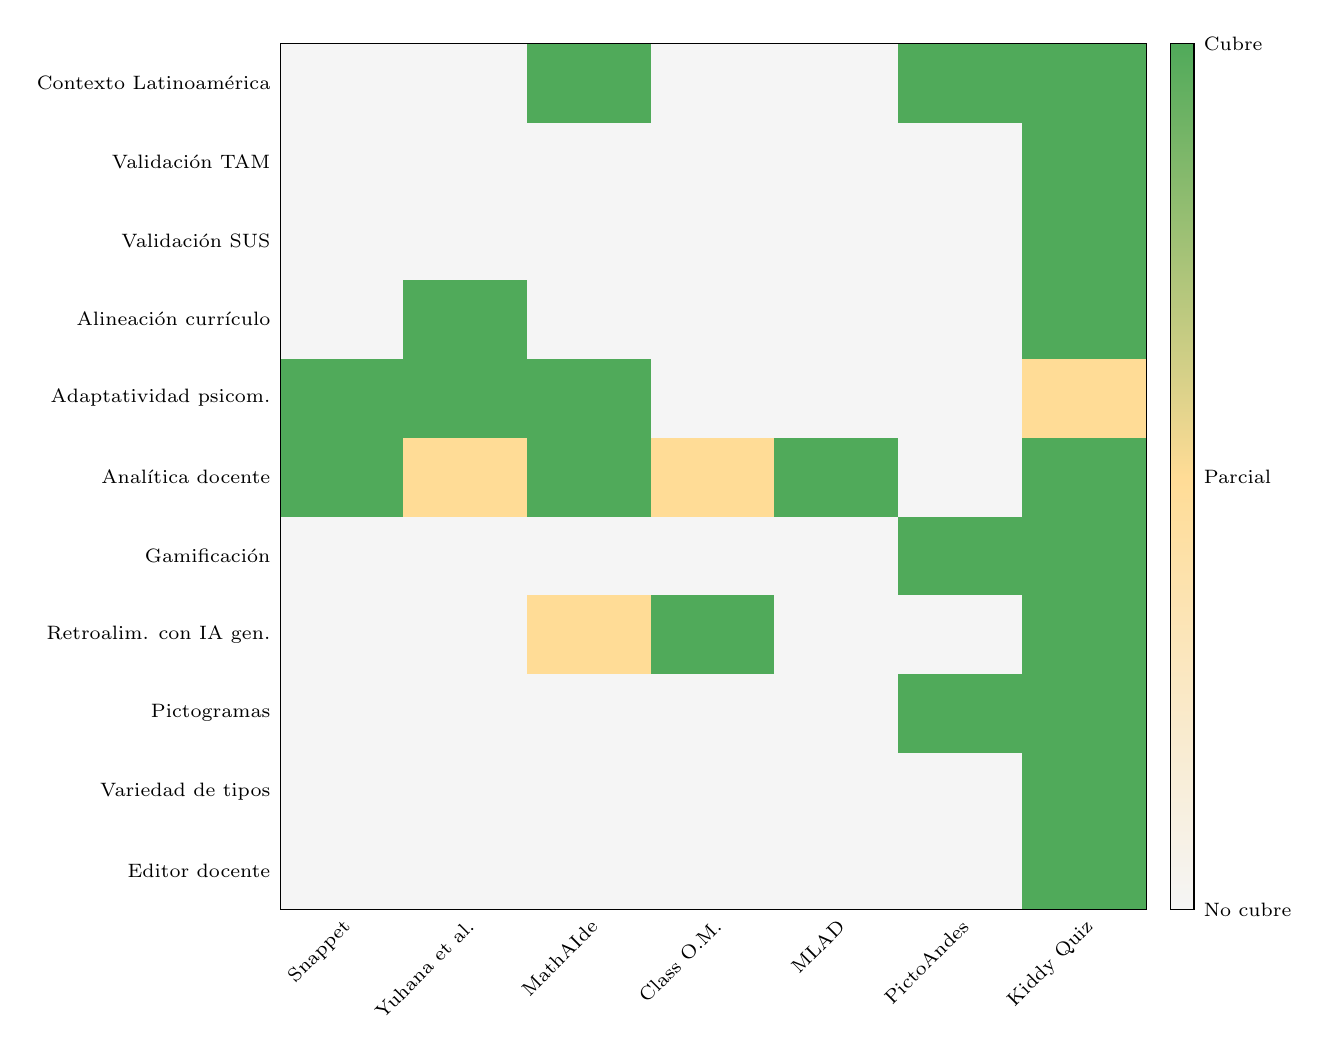
\begin{tikzpicture}
\begin{axis}[
    width=11.0cm,
    height=11cm,
    scale only axis,
    colormap={cobertura}{
        rgb255(0cm)=(245,245,245);
        rgb255(0.5cm)=(255,220,150);
        rgb255(1cm)=(80,170,90)
    },
    point meta min=0, point meta max=1,
    colorbar,
    colorbar style={
        width=0.3cm,
        ytick={0,0.5,1},
        yticklabels={No cubre, Parcial, Cubre},
        ticklabel style={font=\scriptsize}
    },
    xmin=-0.5, xmax=6.5,
    ymin=-0.5, ymax=10.5,
    xtick={0,1,2,3,4,5,6},
    ytick={0,1,2,3,4,5,6,7,8,9,10},
    xticklabels={
        Snappet,
        Yuhana et al.,
        MathAIde,
        Class O.M.,
        MLAD,
        PictoAndes,
        Kiddy Quiz
    },
    yticklabels={
        Editor docente,
        Variedad de tipos,
        Pictogramas,
        Retroalim. con IA gen.,
        Gamificación,
        Analítica docente,
        Adaptatividad psicom.,
        Alineación currículo,
        Validación SUS,
        Validación TAM,
        Contexto Latinoamérica
    },
    xticklabel style={rotate=45, anchor=north east, font=\scriptsize, inner sep=2pt},
    yticklabel style={font=\scriptsize},
    enlargelimits=false,
    axis on top,
    point meta=explicit,
    tick style={draw=none}
]
\addplot [
    matrix plot*,
    mesh/cols=7,
    point meta=explicit
] table [meta=z] {
x  y  z
0  0  0
1  0  0
2  0  0
3  0  0
4  0  0
5  0  0
6  0  1
0  1  0
1  1  0
2  1  0
3  1  0
4  1  0
5  1  0
6  1  1
0  2  0
1  2  0
2  2  0
3  2  0
4  2  0
5  2  1
6  2  1
0  3  0
1  3  0
2  3  0.5
3  3  1
4  3  0
5  3  0
6  3  1
0  4  0
1  4  0
2  4  0
3  4  0
4  4  0
5  4  1
6  4  1
0  5  1
1  5  0.5
2  5  1
3  5  0.5
4  5  1
5  5  0
6  5  1
0  6  1
1  6  1
2  6  1
3  6  0
4  6  0
5  6  0
6  6  0.5
0  7  0
1  7  1
2  7  0
3  7  0
4  7  0
5  7  0
6  7  1
0  8  0
1  8  0
2  8  0
3  8  0
4  8  0
5  8  0
6  8  1
0  9  0
1  9  0
2  9  0
3  9  0
4  9  0
5  9  0
6  9  1
0  10  0
1  10  0
2  10  1
3  10  0
4  10  0
5  10  1
6  10  1
};
\end{axis}
\end{tikzpicture}
\caption{Mapa de cobertura de las dimensiones críticas de evaluación por competencias en educación primaria. Cada celda indica el grado de cobertura de la dimensión por parte de la herramienta correspondiente: verde indica cobertura plena, amarillo cobertura parcial y gris ausencia documentada en la literatura revisada.}
\label{fig:cobertura}
\end{figure}
\elaboracion

\subsubsection{Vacíos identificados y posicionamiento de la propuesta}

El examen sistemático de los veintidós trabajos analizados, sintetizado en la Tabla~\ref{tab:comparativo} y la Figura~\ref{fig:cobertura}, revela cuatro limitaciones estructurales que, en conjunto, configuran el espacio de oportunidad que Kiddy Quiz busca ocupar:

\textbf{(1) Disociación entre evaluación formativa y accesibilidad cognitiva.} Las herramientas con sólida fundamentación evaluativa (Snappet, Yuhana et al., Tian et al., MathAIde, los estudios de Tirado-Olivares y Rodríguez-Martínez) carecen de dispositivos de accesibilidad cognitiva orientados a la primera infancia escolar. Recíprocamente, las soluciones que sí incorporan pictogramas y adaptación visual (PictoAndes, TEVI, los sistemas analizados por Tönsing et al.) se sitúan fuera del dominio evaluativo. Kiddy Quiz integra ambas dimensiones por primera vez en el contexto andino, apoyándose en la evidencia de eficacia de ARASAAC documentada por Zurita Díaz et al.

\textbf{(2) Limitada capacidad para la creación docente integrada de instrumentos heterogéneos.} Las plataformas analizadas operan, en su mayoría, sobre bancos de preguntas curados externamente o sobre formatos de evaluación restringidos (ejercicios aritméticos en Snappet, pruebas adaptativas en Yuhana et al., tareas Moodle en los trabajos del grupo de Castilla-La Mancha, ejercicios escritos en papel en MathAIde). La capacidad de que un docente diseñe, dentro del mismo entorno, evaluaciones que combinen opción múltiple, unión de columnas, secuencias y respuestas con apoyo pictográfico no aparece reportada en ningún sistema revisado.

\textbf{(3) Incipiente integración de IA generativa con marcos curriculares por competencias.} Aunque \textit{Class Optimization Master} \cite{zheng2023genai} demuestra la viabilidad técnica y motivacional de la retroalimentación generativa en primaria, ninguno de los trabajos revisados documenta integración explícita y verificable con un marco curricular nacional por competencias. Kiddy Quiz cierra esta brecha mediante la articulación operativa de Gemini~2.5~Flash con el Currículo Priorizado con Énfasis en Competencias del Ministerio de Educación del Ecuador.

\textbf{(4) Ausencia de validación combinada SUS--TAM en plataformas de evaluación infantil.} La revisión muestra que las herramientas analizadas se validan, en el mejor de los casos, mediante usabilidad técnica (WCAG~2.1 en PictoAndes) o eficacia pedagógica (rendimiento académico en Faber et al.\ y Snappet, motivación matemática en Class Optimization Master), pero ninguna documenta validación combinada de usabilidad percibida (\textit{System Usability Scale}, SUS) y aceptación tecnológica (\textit{Technology Acceptance Model}, TAM) con docentes y estudiantes de educación básica elemental como muestras independientes. Kiddy Quiz aporta esta evidencia con SUS de 87,7 (estudiantes) y 81,0 (docentes), y TAM con índice de Intención de Uso de 4,93/5.

En esencia, la revisión sistemática presentada ---visualmente respaldada por el flujo PRISMA de la Figura~\ref{fig:prisma}, el comparativo funcional de la Tabla~\ref{tab:comparativo} y el mapa de cobertura de la Figura~\ref{fig:cobertura}--- evidencia que las herramientas existentes en el estado del arte abordan de manera parcial e inconexa los desafíos de la evaluación por competencias en educación primaria. La propuesta desarrollada en el presente proyecto tecnológico, cuyo funcionamiento se detalla en el Capítulo~IV, integra de manera articulada las cuatro dimensiones identificadas como vacíos: editor docente para creación de evaluaciones heterogéneas, retroalimentación motivacional generada por IA alineada al currículo nacional, accesibilidad cognitiva mediante ARASAAC, y validación empírica combinada SUS--TAM en el contexto educativo ecuatoriano. Este conjunto integrado, no presente en ninguno de los veintidós trabajos analizados, sitúa a Kiddy Quiz en la frontera del conocimiento aplicado en evaluación educativa tecnológica para la infancia.